\documentclass{sig-alternate}
\usepackage{balance,bm,subfigure,commath,amsfonts,algorithmic,algorithm,graphicx,times,cite,multicol,multirow,tabularx,amsmath,booktabs,array,marvosym,morefloats}
\usepackage[rgb]{xcolor}
\usepackage{epsfig,times,amsthm,amssymb}
%\usepackage{caption}
\usepackage[online]{threeparttable}
\usepackage{bm}
\usepackage[bookmarks=false]{hyperref}
\usepackage{breqn,lipsum,pbox,commath,fancyhdr}
\usepackage[sort&compress]{natbib} 
\setlength{\textfloatsep}{12pt plus 2.0pt minus 4.0pt} 
\setlength{\bibsep}{0ex}
\usepackage[skip=3pt]{caption}
\def\baselinestretch{0.96}
\linespread{0.96}

\begin{document}
 
\title{Do we really need complicated scalarization techniques for MaOP ?}

\maketitle
\begin{abstract} 
Recently, decomposition based approaches are gaining popularity in dealing many-objective optimization problems. In such approaches, the MaOP is decomposed into several single-objective sub-problems and solved simultaneously guided by a set of predefined, uniformly distributed reference vectors. The reference vectors are normally constructed by joining a set of uniformly sampled points to the ideal point. Till date, there exists numerous such decomposition based approaches utilizing various scalarization techniques to achieve a balance between convergence and diversity in the context of many-objective optimization problems. This paper uses an existing yet simple scalarization technique in the context of a decomposition based approach and compare the performance with some existing well known algorithms for many objective optimization. In this context, we aim to show that simple scalarization technique works well for normal and inverted instances of DTLZ1-DTLZ4 and WFG1-WFG9 problems. In this paper we objectively compare the performances delivered by the proposed approach with various state of the art approaches on 3, 5, 8 and 10 objective instances of the above problems. The results clearly highlight the benefits of such a simple scalarization technique on this class of problems in the context of decomposition based evolutionary approaches.\\ 
\end{abstract}

\keywords{Modified distance based ranking, Decomposition, Many-objective optimization, Reference directions, Adaptive} 


\section{Introduction} 

In many real world design problems, there is a need to simultaneously optimize multiple conflicting objectives. Optimization in presence of four or more objectives is commonly referred to as many-objective optimization problem~(MaOP) and the area has received significant research attention in recent years due to its unique set of challenges. The particular focus has been on \emph{decomposition} based approaches, where the MaOP is divided into a set of single-objective sub-problems and collectively solved using a set of uniformly distributed reference vectors. Multi-objective evolutionary algorithm based on decomposition~(MOEA/D)~\cite{zhang2007moead} is among the most well-known algorithm in this class. Subsequently, the benefits of decomposition and its potential use for many-objective optimization soon became apparent, and a number of further developments leveraged this idea~\cite{trivedisurvey}. In the decomposition based approaches, typically a set of uniformly distributed points are generated using systematic sampling~\cite{das1998normal} on an hyperplane with unit intercepts in each objective axis. This is represented by the plane $\sum^{M}_i{f_i}=1$ in the normalized $M$-objective space. Lines joining the ideal point to the above sampled set of points yield the set of reference vectors that are used to define sub-problems and a scalarization function is constructed within each sub-problem such as weighted sum~\cite{miettinen2012nonlinear, Voss2008}, Chebyshev/penalized boundary intersection~(PBI)~\cite{zhang2007moead}, achievement scalarizing function (ASF)~\cite{miettinen2012nonlinear, Yuan2016many}, etc to guide the search.

The scalarization functions convert the multi/many-objective optimization problem into a set of single objective optimization problems, which in turn helps achieving better balance between convergence and diversity compared to pareto dominance based approaches. However, it is important to note that not all scalarizing functions can guarantee that all Pareto optimal solutions will be obtainable \cite{miettinen2012nonlinear}. Hence, a stable scalarizing function will be able to obtain a unique Pareto optimal solution for every sub-problem \cite{giakiozis2015}. Substantial amount of research has gone into designing suitable scalarizing functions to solve a MaOP. 

Let us consider a three objective DTLZ1 \cite{deb2005scalable} problem and its recently improvised ``minus'' version proposed in \cite{ishibuchi2016inverse}, denoted as DTLZ\textsuperscript{-1}. The DTLZ\textsuperscript{-1} problem is constructed by maximizing each objective instead of minimizing them. Consequently, the problem can be solved as minimization of negative of each of the original DTLZ1 objectives~(hence the nomenclature). The POF of the minus problem is ``inverted '' compared to that of the original DTLZ1, in a sense that all vertices of the POF are symmetrically located on the objective planes rather than the objective axes. If one opts to use a decomposition based algorithm to solve DTLZ1 with reference vectors originating from the ideal point~(without any reference vector adaptation), the distribution of the obtained solutions will look like the one presented in Figure \ref{fig:dtlz1pbi}. Instead, if the same approach is used to solve the DTLZ\textsuperscript{-1} problem, the results obtained would look similar to the one presented in Figure \ref{fig:dtlz1mpbi}. Clearly, for the first problem~(DTLZ1), the solutions are well distributed, while for the other(minus DTLZ1), the distribution is far from satisfactory. On the other hand, if one opted to use reference directions from nadir point for both problems, the solutions would be far from satisfactory for the original DTLZ1, while for the DTLZ\textsuperscript{-1} it would deliver a well distributed set of solutions, as depicted in Figures \ref{fig:dtlz1ipbi} and Figure \ref{fig:dtlz1mipbi} respectively.

\begin{figure*}[!htb]
\centering
\subfigure[]{\label{fig:dtlz1pbi}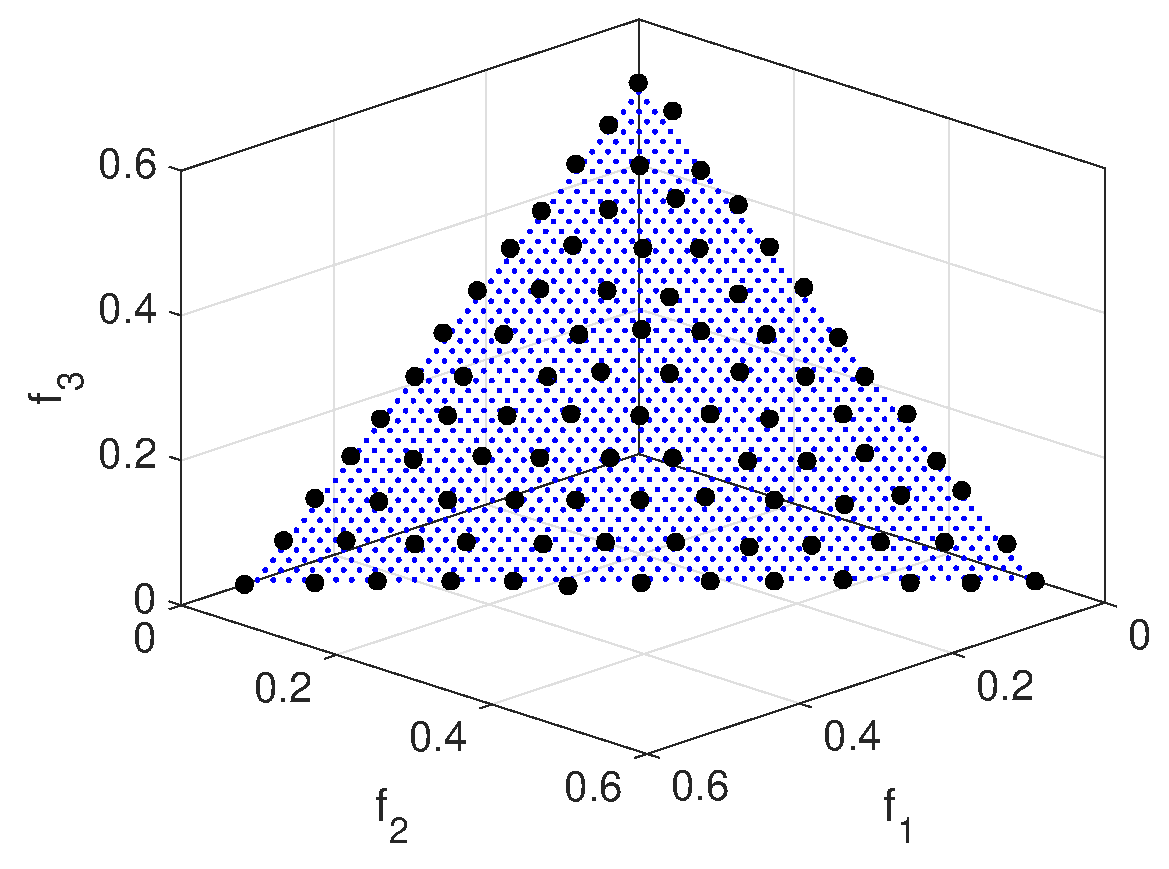
\includegraphics[scale = .22]{Figures/dtlz1_PBI.eps}}
\subfigure[]{\label{fig:dtlz1mpbi}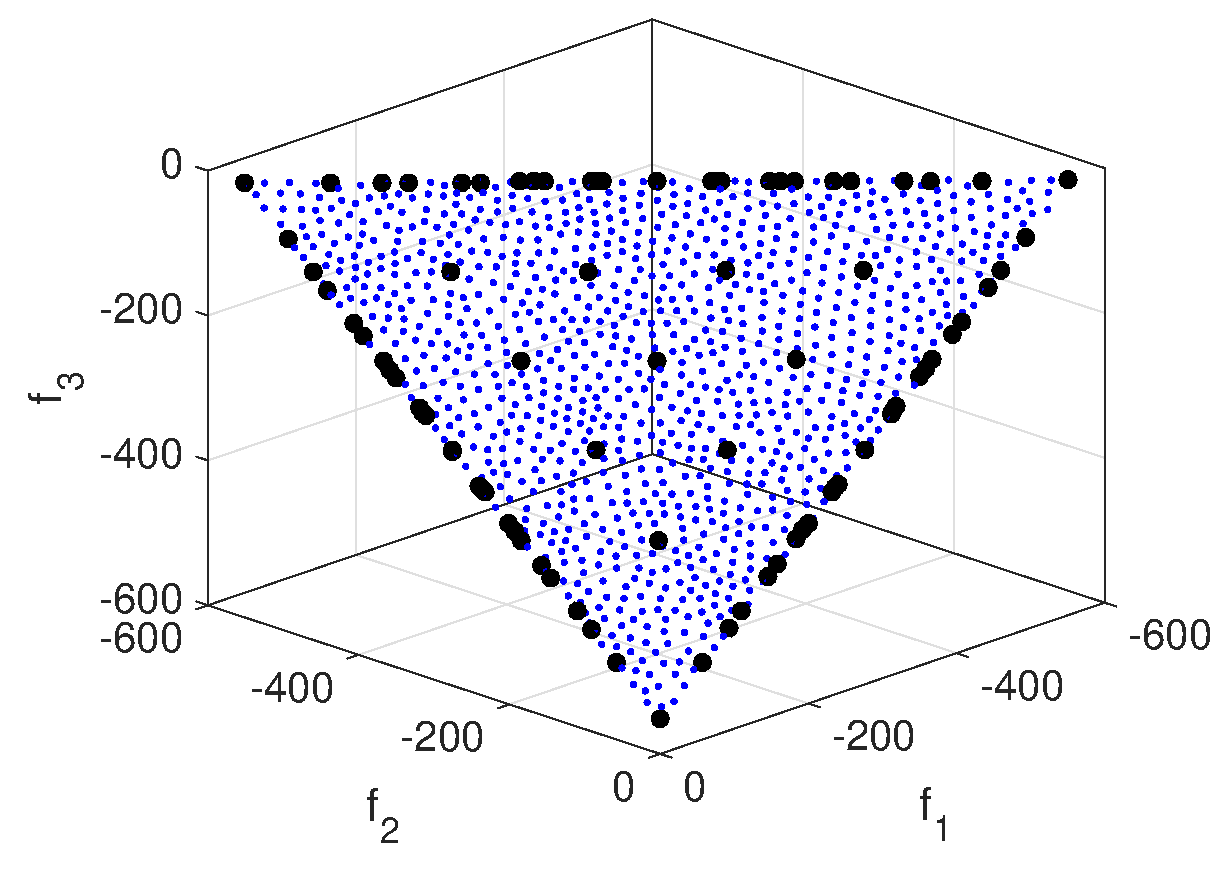
\includegraphics[scale = .22]{Figures/dtlz1m_PBI.eps}}
\subfigure[]{\label{fig:dtlz1ipbi}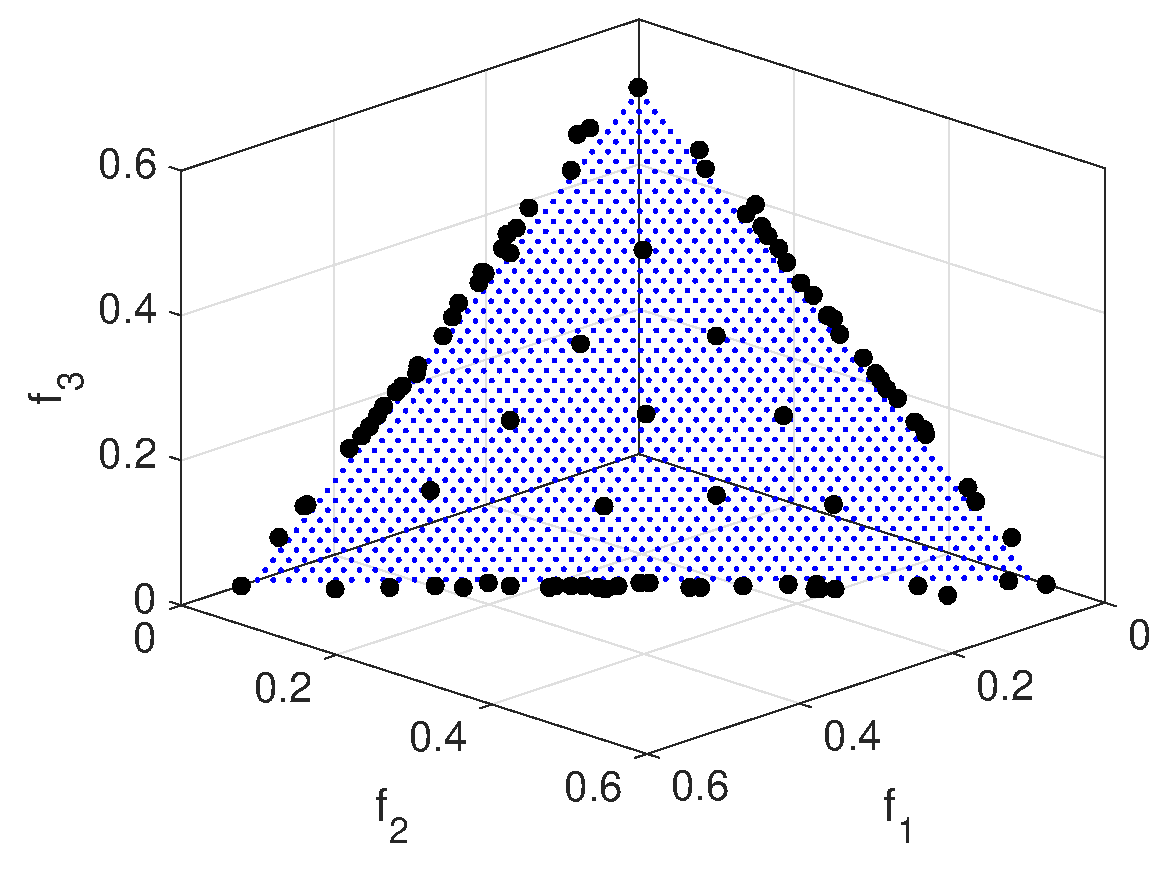
\includegraphics[scale = .22]{Figures/dtlz1_IPBI.eps}}
\subfigure[]{\label{fig:dtlz1mipbi}\includegraphics[scale = .22]{Figures/dtlz1m_IPBI.eps}}
\label{fig:rationale}
\caption{Final distribution: (a) DTLZ1 (ideal point), (b) Minus DTLZ1 (ideal point) (c) DTLZ1 (nadir point),  (d) Minus DTLZ1 (nadir point)}
\end{figure*}

In this paper, we aim to exploit the complementary strengths of these two sets of reference vectors, and to this end, propose and study an algorithm that uses both. Section~\ref{sec:proapp} introduces the proposed approach and outlines the details of individual components. Section \ref{sec:expset} and Section \ref{sec:perf} outlines the parameter settings for the selected set of problems and the performance measures chosen for comparison. In Section~\ref{sec:resdis}, performance of the proposed approach is objectively compared with existing state-of-the-art algorithms on a selected set of test problems. The results clearly highlight that such a scheme is more robust than existing non-adaptive algorithms that rely on a single set of reference directions. Finally, a summary of the work and some potential directions for future development are discussed in Section \ref{sec:conc}.


\section{Proposed Approach}
\label{sec:proapp}

\label{sec:KHT_sec:2}
A generic unconstrained multi/many-objective optimization problem can be defined as shown in Equation~\ref{eqn:KHT_Eqn:1}.

\begin{equation}
\begin{aligned}
\operatorname{Minimize}\; & f_i(\textbf{x}); i=1,2,.......M \\
\text{Subject to} & \\ 
& \hspace{-0.6cm}\textbf{x}^{L}\le\textbf{x}\le\textbf{x}^{U}\\ 
\label{eqn:KHT_Eqn:1}
\end{aligned}
\end{equation}

\noindent Here, $f_1(\textbf{x})$  to $f_M(\textbf{x})$ are the $M$ objective functions. Without loss of generalization, minimization of each objective is assumed. The upper and lower bounds of the variables are denoted as $\textbf{x}^{U}$ and $\textbf{x}^{L}$. The ideal vector~($Z^I$) can be constructed by identifying minimum of each $M$ objectives. We identify the set of non-dominated solutions and use the maximum values of each objective to define the coordinates of the nadir vector $Z^N$. 

To deal with unconstrained many-objective optimization problems, the following algorithm is proposed and is referred to as Decomposition Based Evolutionary Algorithm using Distance based Ranking (DBEA-DR). The proposed approach is based on a ($\mu$ + $\lambda$) evolutionary model, where $\mu$ parents are recombined to generate $\lambda$ offspring and the \textit{best} $\mu$ solutions are selected as parents for the next generation.The pseudo-code of the proposed method is presented in Algorithm~\ref{alg:ADBEA} and the details of its key components are outlined in the following subsections.

\begin{algorithm}[!ht]\footnotesize
   \caption{DBEA-DR}
   \textbf{Input:} $Gen_{max}$\hspace{1mm}(Total number of generations allowed), $N$\hspace{1mm}(Population size during evolution i.e. $\mu$)
   \begin{algorithmic}[1]
   	\STATE $Gen$ = 0, $j$ = 0
   	\STATE \textbf{Generate} $W$ reference points using Normal Boundary Intersection.
   	\STATE Construct $W$ reference directions by joining origin and $W$ reference points
   	\STATE $P^j$ = \textbf{Initialize}(), $\left|P^j\right| = N_I$ 
   	\STATE \textbf{Evaluate} every objective function of $P^j$
   	\STATE $W_m$ = \textbf{UpdateRef}($W$,$P^j$)
   	\STATE $P^j$ = \textbf{Assign}($W_m$,$P^j$) 	
   	\WHILE{$(Gen\le Gen_{max})$}
   	\STATE $C$ = \textbf{CreateOffspring}($P^j$), $\left|C\right|$ = $N$
   	\STATE \textbf{Evaluate} each objective function of $C$
   	\STATE $W_m$ = \textbf{UpdateRef}($W$,$P^j \cup C$)
   	\STATE $P^{j+1}$ = \textbf{Assign}($W_m$,$P^j \cup C$)   
   	\STATE $Gen$ = $Gen$ + 1
   	\ENDWHILE		
  
	\end{algorithmic}
   \label{alg:ADBEA}
\end{algorithm} 

The highlighted parts of the algorithm are elaborated below:\\
\begin{itemize}
	\item \textbf{Generate}: A structured set of $W$ reference points is generated using the method of systematic sampling~(normal boundary intersection) as outlined in~\cite{KHT_das1998normal}. The approach generates $W$ points on the hyperplane in $M$-objcetive space with a uniform spacing of $\delta=1/H$ with $H$ unique sampling locations along each objective axis. The reference directions are formed by joining the ideal point~(origin in the scaled space) to each of these reference points. In this approach, $N = {H+M-1}\choose{M-1}$ reference directions are generated. However, for larger number of objectives, a two-layered approach is commonly used in the field~(and adopted here) which is defined using $H_1$ and $H_2$ as outlined in \cite{KHT_Li2015dominance}. Such an approach limits the number of reference points from growing exponentially. The two-layered approach generates $N_1 = {H_1+M-1}\choose{M-1}$ points on the boundary and $N_2 = {H_2+M-1}\choose{M-1}$ points inside the hyperplane as shown in Fig~\ref{fig:KHT_Fig:1}. The $j^{th}$ coordinate ($W_j$) of each of the weight vectors in the inside layer generated using \cite{das1998normal} are modified using Equation~\ref{eqn:KHT_Eqn:2}, where $\tau$ = 0.5 is considered \cite{Li2015dominance}.
	
	\begin{equation}
	W_j = \frac{1-\tau}{M} + \tau \times W_j
	\label{eqn:KHT_Eqn:2} 
	\end{equation} 
	
	\begin{figure}[!htb]
		\centering
		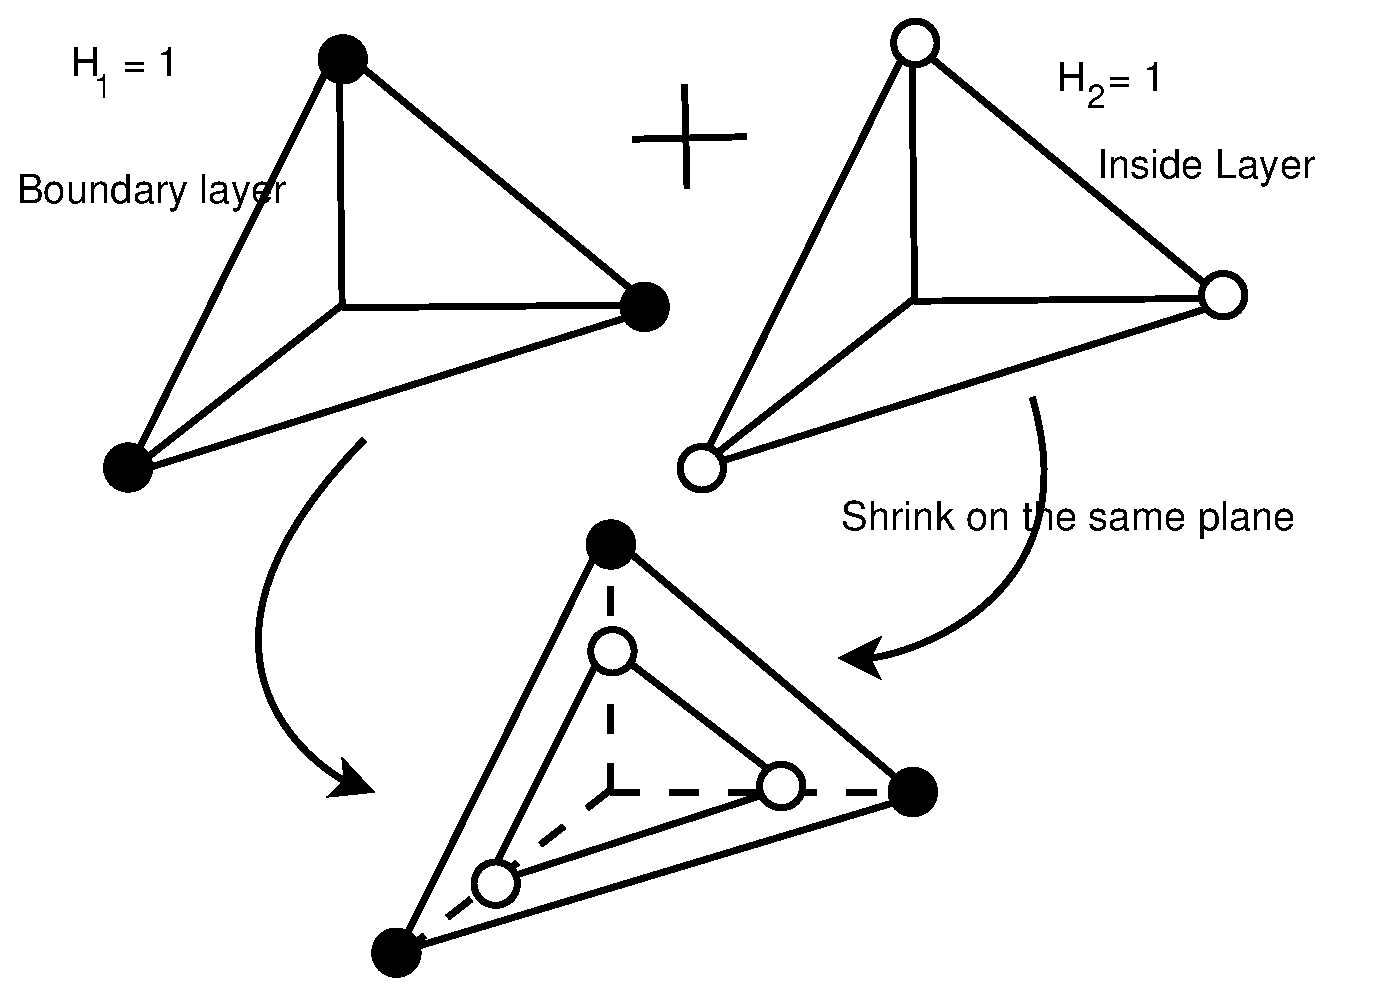
\includegraphics[width=.7\textwidth]{fig1.eps}
		\caption{Structured two-layered set of reference points with $M=3$, $H_1=1$, $H_2=1$. The filled circles represent the reference points generated on the boundary/outside layer, while the hollow circles represent those generated on the inside layer.}
		\label{fig:KHT_Fig:1}
	\end{figure}
	
	\item \textbf{Initialize}: $N$ solutions are initialized within the variable bounds $\textbf{x}^{L}$ and $\textbf{x}^{U}$ using Latin Hypercube Sampling based on ``maximin'' criterion.
	
	\item \textbf{Evaluate}: In this stage, the objective functions are evaluated for all the solutions generated above.
	
	\item \textbf{UpdateRef}: In this stage, the $i^{th}$ reference direction $W^i$ is modified to $W^i_m$ based on the ideal vector ($Z^I$) and nadir vector ($Z^N$) of the combined parent and child population using Equation \ref{eqn:KHT_Eqn:3}. Take note that the proposed approach uses the nadir point of the combined parent, child and archive population as opposed to maximum value of each objective function of parent and child population in the Reference Vector guided Evolutionary Algorithm~\cite{Cheng2016many}. 
	
	\begin{equation}
	(W^i_m)_j = (W^i)_j\times(Z^N - Z^I)_j, \forall~1\le j\le M
	\label{eqn:KHT_Eqn:3}
	\end{equation}
	
	
	\item \textbf{Assign}: In this stage, solutions are assigned to the reference directions. Let the number of solutions to be assigned be denoted by $R$. If the number of solutions to be assigned is more than $N$, the solutions are assigned in each subpopulation using distance based ranking. Take note that, in the assignment process, a sub-population with respect to a reference direction is constructed using the solutions which are closest to that reference direction based on angle measure. If no solutions belong to a sub-population, it is considered empty. Solutions within a non-empty sub-population is sorted based on a metric (modified distance based ranking) value which is obtained by comparing the objective values. The value of the metric for $i^{th}$ solution within a subpopulation of $P$ member is computed as:
	
	\begin{equation}
	DR\_m_i = \sum_{k\neq i}\sum_{j=1}^M max(\{(- f^i_j + f^k_j),0\}) 
	\label{eqn:KHT_Eqn:4}
	\end{equation}
	
	This equation for the $i^{th}$ solution only aggregrates the difference values of objectives with other solutions which are worse than the $i^{th}$ solution.
	
	\item \textbf{CreateOffspring}: The process of creating offspring solutions involves two steps, the identification of participating parents for recombination and the recombination process itself. Both these steps are known to affect the performance and various rationales and recommendations have been suggested in the literature. 
	
	In our approach, each solution is selected as a base parent and its partner is randomly chosen from the rest. Such a scheme offers opportunity to all solutions to act as base parents for generating offspring. We capitalize on the advantages of two commonly used recombination schemes, i.e., differential evolution~(DE) crossover~\cite{das2011de} and simulated binary crossover~(SBX)~\cite{deb2002fast}. At each generation both types of crossover and polynomial mutation are employed for each of the base parents attached to each reference direction i.e. if at the first generation, the first reference direction uses differential evolution crossover, the second reference direction  would use simulated binary crossover and this will be reversed in the second generation. Such an alternation also removes the bias induced by the specific operators. One and two participating parents are identified when using SBX and DE respectively which results in two and one offspring respectively out of which the first offspring is selected.       
	
\end{itemize}

\section{Numerical Experiments}
\label{sec:expset}

In order to objectively compare the performance of the proposed algorithm with published set of results, we adopt settings that were used in the studies~\cite{Deb2014adaptive,ishibuchi2016inverse}. A probability of crossover of 1 and a probability of mutation of $\frac{1}{n}$ ($n$ is the number of variables) \cite{Deb2014adaptive} was used for all problems studied in the paper. The distribution index of crossover was set to $30$ and the distribution index of the mutation was set to $20$ for all problems \cite{Deb2014adaptive}. We have set crossover rate ($CR$) as 1 and scaling factor ($F$) as 0.5 for the differential evolution crossover \cite{das2011de}. Full default precision of MATLAB was used without any rounding/casting of the objectives/variable values. The parameter settings used for various problems are listed below in Table~\ref{tab:params_term_con}. The results of the proposed approach are based on 21 independent runs for all the problems.  

\begin{table}[!htb]
\begin{threeparttable}
\caption{Termination condition used in the study}
\label{tab:params_term_con}
\tabcolsep = 1mm
\begin{tabular}{p{2.5cm}p{.5cm}p{5cm}}
\hline
\textbf{Problems}&\textbf{M}& \textbf{Termination condition ([number of generations(G), population size])}\\
\hline
DTLZ1/DTLZ1\textsuperscript{-1}& 3,5,8 &([400(G),91];[600(G),210];[750(G),156])\\
DTLZ2/DTLZ2\textsuperscript{-1}& 3,5,8 &(250(G),91];[350(G),210];[500(G),156])\\
DTLZ3/DTLZ3\textsuperscript{-1}& 3,5,8 &([1000(G),91];[1000(G),210];[1000(G),156])\\
DTLZ4/DTLZ4\textsuperscript{-1}& 3,5,8 &([600(G),91];[1000(G),210];[1250(G),156])\\
WFG1/WFG1\textsuperscript{-1}-WFG9/WFG9\textsuperscript{-1}& 3,5,8 &([400(G),91];[750(G),210];[1500(G),156])\\
\hline
\end{tabular}
\end{threeparttable}
\end{table}

\subsection{Performance Measures}
\label{sec:perf}

 Inverted generation distance~(IGD) and hypervolume~(HV) are the most common metrics used for an quantitative assessment in the multiobjective optimization domain. Computation of IGD requires a reference POF, while computation of HV requires a reference point. The aspect of uniformity of solutions in the reference set can always be questioned. As for hypervolume, the choice of the reference point used for HV computation is crucial and can adversely affect the interpretations about relative performance~\cite{Yuan2016many,ishibuchi2010many}. For HV computation, there are recent reports that suggest use of a slightly larger than true nadir vector as a reference point~\cite{Yuan2016many,ishibuchi2010many}. In our experiments, we have used the reference point to be 1.1 multiplied by the actual nadir vector for problems, where the nadir vector can be analytically computed. Given a set of solutions and their corresponding objective vectors, we first discard all solutions that are dominated by the reference point. The objective vectors of the remaining solutions are normalized using the ideal and the nadir vector and HV is computed using a reference point which is $1.1^M$ in the normalized space~($M$ is the number of objectives). All HV computations reported in this paper are based on exact method~(WFG algorithm)~\cite{while2012hv}. HV and IGD computations in this paper are based on solutions obtained from the archive (set of all fully evaluated solutions so far) instead of the final population obtained at the end of optimization for all the problems. At first all the non-dominated solutions are collected from the archive. In the next stage, subset of non-dominated solutions are constructed using affinity propagation clustering~\cite{apcluster2011} and used for HV and IGD computation. 

\subsection{Results and Discussion}
\label{sec:resdis}
 
\subsubsection{Normal Problems}

Next we demonstrate the performance of DBEA-DR on 13 unconstrained DTLZ and WFG series problems (DTLZ1-DTLZ4, WFG1-WFG9) and Minus-problems introduced in \cite{ishibuchi2016inverse}: DTLZ1\textsuperscript{-1}-DTLZ4\textsuperscript{-1} and WFG1\textsuperscript{-1}-WFG9\textsuperscript{-1}. These problems are well suited to demonstrate the efficiency of using both $\mathbf{W}^I$ and $\mathbf{W}^N$. The detailed description of the problems and the difficulties in solving them can be found in \cite{ishibuchi2016inverse}. 

\begin{table*}[!htb]\scriptsize
\centering
\renewcommand{\arraystretch}{0.9}
\caption{Mean HV statistics for DTLZ and WFG series problems}
\label{tab:HV}
\tabcolsep = 0.1cm
\begin{tabular}{|c|c|c|c|c|c|c|c|c|c|c|c|}
\noalign{\smallskip}\hline
\textbf{Problem}                & \textbf{M} & \textbf{DBEA-DR} & \textbf{NSGA-III} & \textbf{$\theta$-DEA} & \textbf{MOEA/DD} & \textbf{MOEA/D-PBI} & \textbf{MOEA/D-Tch} & \textbf{MOEA/D-WS} & \textbf{MOEA/D-IPBI} & \textbf{NSGA-II} \\ \hline
\multirow{4}{*}{\textbf{DTLZ1}} & 3          & 1.11657          & 1.11508           & 1.11767               & \textbf{1.11913} & 1.11711             & 1.06842             & 0.39572            & 0.48149              & 1.07411          \\ \cline{2-11} 
& 5          & 1.56068          & 1.57677           & 1.57767               & \textbf{1.57794} & 1.57768             & 1.51186             & 0.50052            & 0.02284              & 0.00000          \\ \cline{2-11} 
& 8          & 2.01262          & 2.13770           & \textbf{2.13788}      & 2.13730          & 2.13620             & 2.05463             & 0.96246            & 1.44289              & 0.00000          \\ \cline{2-11} 
& 10         & 2.52609          & \textbf{2.59280}  & 2.59272               & 2.59260          & 2.59220             & 2.51973             & 1.07913            & 1.90272              & 0.00000          \\ \hline
\multirow{4}{*}{\textbf{DTLZ2}} & 3          & 0.74018          & 0.74336           & 0.74390               & \textbf{0.74445} & 0.74418             & 0.70168             & 0.33187            & 0.33100              & 0.69708          \\ \cline{2-11} 
& 5          & 1.29193          & 1.30317           & 1.30679               & \textbf{1.30778} & 1.30728             & 1.14598             & 0.61944            & 0.27191              & 0.67442          \\ \cline{2-11} 
& 8          & 1.89112          & 1.96916           & 1.97785               & \textbf{1.97862} & 1.97817             & 1.35469             & 0.68315            & 0.54410              & 0.00004          \\ \cline{2-11} 
& 10         & 2.42404          & 2.50878           & 2.51416               & \textbf{2.51509} & 2.51500             & 1.69045             & 0.83883            & 0.64925              & 0.00000          \\ \hline
\multirow{4}{*}{\textbf{DTLZ3}} & 3          & \textbf{0.74358} & 0.73300           & 0.73642               & 0.73944          & 0.73654             & 0.69553             & 0.33026            & 0.31397              & 0.69959          \\ \cline{2-11} 
& 5          & 1.26280          & 1.29894           & 1.30376               & \textbf{1.30638} & 1.30398             & 1.14475             & 0.60143            & 0.00750              & 0.00000          \\ \cline{2-11} 
& 8          & 1.54620          & 1.95007           & 1.96849               & \textbf{1.97162} & 1.74240             & 1.33166             & 0.66684            & 0.29765              & 0.00000          \\ \cline{2-11} 
& 10         & 1.38691          & 2.50727           & 2.51279               & \textbf{2.51445} & 2.50933             & 1.69956             & 0.80348            & 0.52362              & 0.00000          \\ \hline
\multirow{4}{*}{\textbf{DTLZ4}} & 3          & 0.74138          & 0.73221           & 0.71077               & \textbf{0.74484} & 0.48232             & 0.45889             & 0.17191            & 0.23377              & 0.70481          \\ \cline{2-11} 
& 5          & 1.28523          & 1.30839           & \textbf{1.30878}      & 1.30876          & 1.20680             & 1.00426             & 0.42941            & 0.33457              & 1.00881          \\ \cline{2-11} 
& 8          & 1.90844          & 1.98025           & 1.98078               & \textbf{1.98083} & 1.86439             & 1.35100             & 0.71296            & 0.53303              & 0.00000          \\ \cline{2-11} 
& 10         & 2.45313          & 2.51524           & \textbf{2.51539}      & 2.51532          & 2.43536             & 1.56890             & 0.95488            & 0.64498              & 0.00000          \\ \hline
\multirow{4}{*}{\textbf{WFG1}}  & 3          & 0.50294          & 0.65088           & 0.70151               & 0.69393          & 0.67291             & \textbf{0.92204}    & 0.73804            & 0.81622              & 0.75944          \\ \cline{2-11} 
& 5          & 0.68580          & 0.85608           & 1.14844               & 1.23809          & 1.34797             & \textbf{1.51824}    & 1.36724            & 1.36241              & 1.03120          \\ \cline{2-11} 
& 8          & 0.91126          & 1.36206           & 1.88297               & 1.91925          & 1.73875             & \textbf{2.05117}    & 1.85604            & 1.75472              & 1.51083          \\ \cline{2-11} 
& 10         & 1.10780          & 2.22078           & 2.38349               & 2.37705          & 1.78435             & \textbf{2.46470}    & 2.27031            & 2.18237              & 2.38032          \\ \hline
\multirow{4}{*}{\textbf{WFG2}}  & 3          & 1.22597          & 1.22359           & \textbf{1.22945}      & 1.22193          & 1.11888             & 1.12990             & 1.12266            & 1.16687              & 1.20760          \\ \cline{2-11} 
& 5          & 1.57110          & \textbf{1.59770}  & 1.59708               & 1.55672          & 1.52205             & 1.58417             & 1.42821            & 1.42081              & 1.58790          \\ \cline{2-11} 
& 8          & 2.12451          & \textbf{2.13629}  & 2.12442               & 2.04619          & 2.01678             & 2.13569             & 2.11651            & 2.11529              & 2.13214          \\ \cline{2-11} 
& 10         & 2.58524          & 2.58890           & 2.57778               & 2.48332          & 2.45715             & \textbf{2.58891}    & 2.57478            & 2.57367              & 2.58882          \\ \hline
\multirow{4}{*}{\textbf{WFG3}}  & 3          & \textbf{0.98265} & 0.81929           & 0.81556               & 0.77295          & 0.75364             & 0.80041             & 0.48971            & 0.74146              & 0.82967          \\ \cline{2-11} 
& 5          & \textbf{1.38769} & 1.01000           & 1.02782               & 0.95386          & 0.89357             & 0.88322             & 0.71619            & 0.93099              & 1.06314          \\ \cline{2-11} 
& 8          & \textbf{1.86632} & 1.21146           & 1.11348               & 1.15306          & 0.74674             & 1.27479             & 0.92248            & 1.41331              & 1.41857          \\ \cline{2-11} 
& 10         & \textbf{2.33286} & 1.55771           & 1.55919               & 1.37737          & 0.55186             & 1.69917             & 1.13233            & 1.72878              & 1.76576          \\ \hline
\multirow{4}{*}{\textbf{WFG4}}  & 3          & 0.70356          & 0.72867           & \textbf{0.72949}      & 0.72031          & 0.68710             & 0.66650             & 0.34131            & 0.63483              & 0.67605          \\ \cline{2-11} 
& 5          & 1.19012          & 1.28496           & \textbf{1.28736}      & 1.26067          & 1.15695             & 1.01300             & 0.71180            & 1.04810              & 1.07969          \\ \cline{2-11} 
& 8          & 1.73811          & 1.96402           & \textbf{1.96426}      & 1.83751          & 1.19841             & 1.33398             & 0.95883            & 1.45141              & 1.40330          \\ \cline{2-11} 
& 10         & 2.26378          & 2.50322           & \textbf{2.50376}      & 2.22383          & 1.43393             & 1.49165             & 1.20197            & 1.74551              & 1.70402          \\ \hline
\multirow{4}{*}{\textbf{WFG5}}  & 3          & 0.67828          & 0.68658           & \textbf{0.68706}      & 0.67698          & 0.65668             & 0.61681             & 0.27764            & 0.58174              & 0.65059          \\ \cline{2-11} 
& 5          & 1.17570          & 1.22187           & \textbf{1.22209}      & 1.18965          & 1.11627             & 0.93276             & 0.58164            & 0.96542              & 1.06695          \\ \cline{2-11} 
& 8          & 1.76351          & 1.84995           & \textbf{1.85027}      & 1.71196          & 1.27483             & 1.18970             & 0.96591            & 1.33675              & 1.39529          \\ \cline{2-11} 
& 10         & 2.27006          & 2.34640           & \textbf{2.34644}      & 2.07711          & 1.53615             & 1.35553             & 1.18471            & 1.57386              & 1.61976          \\ \hline
\multirow{4}{*}{\textbf{WFG6}}  & 3          & 0.66788          & 0.68696           & \textbf{0.68698}      & 0.67923          & 0.65655             & 0.62307             & 0.28542            & 0.58469              & 0.64111          \\ \cline{2-11} 
& 5          & 1.13737          & 1.21978           & \textbf{1.22284}      & 1.19424          & 1.04043             & 0.93460             & 0.55026            & 0.97587              & 1.01175          \\ \cline{2-11} 
& 8          & 1.60951          & \textbf{1.84625}  & 1.84330               & 1.69055          & 0.71742             & 1.17924             & 0.63171            & 1.21597              & 1.27938          \\ \cline{2-11} 
& 10         & 1.97622          & 2.32660           & \textbf{2.32759}      & 2.01837          & 0.82027             & 1.44519             & 0.77606            & 1.48368              & 1.59677          \\ \hline
\multirow{4}{*}{\textbf{WFG7}}  & 3          & 0.72079          & 0.72894           & \textbf{0.73099}      & 0.72126          & 0.61145             & 0.66659             & 0.33309            & 0.62859              & 0.68591          \\ \cline{2-11} 
& 5          & 1.23202          & 1.29190           & \textbf{1.29548}      & 1.25983          & 1.07723             & 1.01449             & 0.63899            & 1.04794              & 0.97811          \\ \cline{2-11} 
& 8          & 1.80241          & 1.97138           & \textbf{1.97353}      & 1.82024          & 0.83439             & 1.30773             & 0.71170            & 1.45307              & 1.22911          \\ \cline{2-11} 
& 10         & 2.24220          & 2.50754           & \textbf{2.50858}      & 2.25713          & 0.95972             & 1.59993             & 0.97177            & 1.73385              & 1.59601          \\ \hline
\multirow{4}{*}{\textbf{WFG8}}  & 3          & 0.63543          & 0.66560           & \textbf{0.66687}      & 0.65741          & 0.62986             & 0.61394             & 0.24450            & 0.26792              & 0.61230          \\ \cline{2-11} 
& 5          & 1.07350          & 1.18225           & \textbf{1.18354}      & 1.15376          & 0.95660             & 0.60364             & 0.46673            & 0.82273              & 0.96648          \\ \cline{2-11} 
& 8          & 1.30584          & 1.75970           & \textbf{1.76647}      & 1.70621          & 0.30471             & 1.20786             & 0.67808            & 1.24044              & 1.28486          \\ \cline{2-11} 
& 10         & 1.74660          & 2.28203           & \textbf{2.28502}      & 2.10729          & 0.27470             & 1.60952             & 0.82704            & 1.57781              & 1.69433          \\ \hline
\multirow{4}{*}{\textbf{WFG9}}  & 3          & 0.66696          & 0.67519           & \textbf{0.67978}      & 0.67146          & 0.57864             & 0.62177             & 0.25170            & 0.51403              & 0.62199          \\ \cline{2-11} 
& 5          & 1.15289          & 1.21058           & \textbf{1.22122}      & 1.15493          & 1.02426             & 0.78608             & 0.53143            & 0.94420              & 0.92841          \\ \cline{2-11} 
& 8          & 1.69746          & 1.80911           & \textbf{1.83678}      & 1.60407          & 0.97800             & 1.23897             & 0.72454            & 1.18318              & 1.07824          \\ \cline{2-11} 
& 10         & 2.17765          & 2.34332           & \textbf{2.36516}      & 1.92977          & 1.15138             & 1.59168             & 0.86178            & 1.49927              & 1.42611          \\ \hline
\end{tabular}
\end{table*}

\begin{table*}[!htb]\scriptsize
	\centering
	\renewcommand{\arraystretch}{0.9}
	\caption{Mean IGD statistics for DTLZ and WFG series problems}
	\label{tab:IGD}
	\tabcolsep = 0.1cm
	\begin{tabular}{|c|c|c|c|c|c|c|c|c|c|c|c|}
		\noalign{\smallskip}\hline
		\textbf{Problem}                & \textbf{M} & \textbf{DBEA-DR} & \textbf{NSGA-III} & \textbf{$\theta$-DEA} & \textbf{MOEA/DD} & \textbf{MOEA/D-PBI} & \textbf{MOEA/D-Tch} & \textbf{MOEA/D-WS} & \textbf{MOEA/D-IPBI} & \textbf{NSGA-II} \\ \hline
		\multirow{4}{*}{\textbf{DTLZ1}} & 3          & \textbf{0.04085} & 0.04362           & 0.04170               & 0.04138          & 0.04175             & 0.06082             & 0.50173            & 0.42397              & 0.06481          \\ \cline{2-11} 
		& 5          & \textbf{0.10797} & 0.11308           & 0.11125               & 0.11110          & 0.11128             & 0.22189             & 0.73685            & 6.52117              & 19.87954         \\ \cline{2-11} 
		& 8          & 0.21661          & 0.17984           & \textbf{0.17513}      & 0.17541          & 0.17601             & 0.23603             & 0.72480            & 0.52039              & 75.18619         \\ \cline{2-11} 
		& 10         & 0.20406          & 0.19094           & \textbf{0.18527}      & 0.18552          & 0.18611             & 0.23786             & 0.78417            & 0.49928              & 77.22337         \\ \hline
		\multirow{4}{*}{\textbf{DTLZ2}} & 3          & \textbf{0.05410} & 0.05799           & 0.05804               & 0.05801          & 0.05800             & 0.07318             & 0.54279            & 0.54641              & 0.07182          \\ \cline{2-11} 
		& 5          & \textbf{0.16794} & 0.19403           & 0.19363               & 0.19368          & 0.19368             & 0.32648             & 0.69062            & 0.93890              & 0.31393          \\ \cline{2-11} 
		& 8          & \textbf{0.37975} & 0.40062           & 0.39802               & 0.39575          & 0.39572             & 0.46026             & 0.94291            & 0.99204              & 1.90946          \\ \cline{2-11} 
		& 10         & \textbf{0.43399} & 0.46752           & 0.46462               & 0.46145          & 0.46120             & 0.53319             & 1.00370            & 1.05344              & 2.15108          \\ \hline
		\multirow{4}{*}{\textbf{DTLZ3}} & 3          & \textbf{0.05351} & 0.06261           & 0.05908               & 0.05824          & 0.05848             & 0.07349             & 0.54419            & 0.54800              & 0.07194          \\ \cline{2-11} 
		& 5          & \textbf{0.18360} & 0.19601           & 0.19496               & 0.19384          & 0.19400             & 0.32551             & 0.70566            & 40.98681             & 116.19480        \\ \cline{2-11} 
		& 8          & 0.45803          & 0.41225           & 0.40224               & \textbf{0.39694} & 0.46660             & 0.47438             & 0.94647            & 1.23378              & 348.09573        \\ \cline{2-11} 
		& 10         & 0.66578          & 0.46843           & 0.46545               & \textbf{0.46165} & 0.46321             & 0.53973             & 1.01331            & 1.12693              & 308.79409        \\ \hline
		\multirow{4}{*}{\textbf{DTLZ4}} & 3          & \textbf{0.05408} & 0.07550           & 0.10791               & 0.05800          & 0.45495             & 0.47158             & 0.83789            & 0.71489              & 0.07012          \\ \cline{2-11} 
		& 5          & \textbf{0.17325} & 0.19378           & 0.19373               & 0.19372          & 0.33507             & 0.45264             & 0.82880            & 0.89434              & 0.22875          \\ \cline{2-11} 
		& 8          & 0.39938          & 0.39672           & 0.39597               & \textbf{0.39534} & 0.53322             & 0.64479             & 0.95178            & 1.00074              & 2.11783          \\ \cline{2-11} 
		& 10         & \textbf{0.45677} & 0.46302           & 0.46191               & 0.46074          & 0.56608             & 0.61814             & 0.99026            & 1.05641              & 2.33543          \\ \hline
		\multirow{4}{*}{\textbf{WFG1}}  & 3          & 0.37862          & 0.21258           & 0.18074               & 0.18377          & 0.20233             & \textbf{0.07600}    & 0.20087            & 0.15597              & 0.16604          \\ \cline{2-11} 
		& 5          & 0.38576          & 0.29117           & 0.20606               & 0.17134          & 0.19663             & \textbf{0.08683}    & 0.18288            & 0.18297              & 0.26815          \\ \cline{2-11} 
		& 8          & 0.38956          & 0.16839           & \textbf{0.07692}      & 0.06678          & 0.08509             & 0.08045             & 0.10808            & 0.12427              & 0.33417          \\ \cline{2-11} 
		& 10         & 0.36936          & 0.08868           & 0.09112               & \textbf{0.07619} & 0.14610             & 0.10095             & 0.10556            & 0.11972              & 0.23599          \\ \hline
		\multirow{4}{*}{\textbf{WFG2}}  & 3          & 0.31750          & 0.04072           & \textbf{0.03577}      & 0.04866          & 0.08872             & 0.08739             & 0.17910            & 0.12579              & 0.05805          \\ \cline{2-11} 
		& 5          & 0.07906          & 0.05691           & \textbf{0.05685}      & 0.08325          & 0.10423             & 0.15136             & 0.21243            & 0.20765              & 0.12767          \\ \cline{2-11} 
		& 8          & 0.29646          & \textbf{0.07015}  & 0.08495               & 0.09183          & 0.09860             & 0.11937             & 0.13764            & 0.13030              & 0.19386          \\ \cline{2-11} 
		& 10         & 0.26440          & \textbf{0.05969}  & 0.08920               & 0.09114          & 0.09578             & 0.11840             & 0.13169            & 0.12416              & 0.19704          \\ \hline
		\multirow{4}{*}{\textbf{WFG3}}  & 3          & \textbf{0.11423} & 0.15399           & 0.28832               & 0.05425          & 0.03745             & 0.04070             & 0.20844            & 0.19232              & 0.05006          \\ \cline{2-11} 
		& 5          & 0.14467          & \textbf{0.09697}  & 0.12176               & 0.12018          & 0.08618             & 0.15235             & 0.34998            & 0.28723              & 0.10195          \\ \cline{2-11} 
		& 8          & 0.20164          & 0.23351           & 0.56029               & \textbf{0.14305} & 0.22451             & 0.33536             & 0.56095            & 0.43524              & 0.15998          \\ \cline{2-11} 
		& 10         & 0.20538          & 0.16754           & 0.41979               & \textbf{0.15640} & 0.31725             & 0.39634             & 0.57148            & 0.55067              & 0.16206          \\ \hline
		\multirow{4}{*}{\textbf{WFG4}}  & 3          & \textbf{0.05942} & 0.05818           & 0.05823               & 0.07217          & 0.07700             & 0.09484             & 0.52334            & 0.25250              & 0.07274          \\ \cline{2-11} 
		& 5          & \textbf{0.16924} & 0.19213           & 0.19223               & 0.26733          & 0.30864             & 0.41147             & 0.63375            & 0.42761              & 0.18244          \\ \cline{2-11} 
		& 8          & \textbf{0.36754} & 0.39954           & 0.39905               & 0.51790          & 0.72445             & 0.51843             & 0.85709            & 0.59237              & 0.37909          \\ \cline{2-11} 
		& 10         & \textbf{0.41973} & 0.46687           & 0.46624               & 0.66822          & 0.84257             & 0.58032             & 0.92412            & 0.70445              & 0.45848          \\ \hline
		\multirow{4}{*}{\textbf{WFG5}}  & 3          & \textbf{0.06080} & 0.06216           & 0.06212               & 0.07543          & 0.07569             & 0.10004             & 0.52875            & 0.24320              & 0.07718          \\ \cline{2-11} 
		& 5          & \textbf{0.16315} & 0.18937           & 0.18935               & 0.25529          & 0.29036             & 0.40381             & 0.65914            & 0.41589              & 0.18139          \\ \cline{2-11} 
		& 8          & \textbf{0.36496} & 0.39141           & 0.39123               & 0.51273          & 0.67067             & 0.51038             & 0.81440            & 0.48871              & 0.36793          \\ \cline{2-11} 
		& 10         & \textbf{0.41725} & 0.45671           & 0.45638               & 0.65521          & 0.80237             & 0.56802             & 0.88882            & 0.55651              & 0.45670          \\ \hline
		\multirow{4}{*}{\textbf{WFG6}}  & 3          & 0.06614          & 0.06237           & \textbf{0.06236}      & 0.07542          & 0.08158             & 0.09964             & 0.53091            & 0.24512              & 0.08111          \\ \cline{2-11} 
		& 5          & \textbf{0.17112} & 0.18939           & 0.18942               & 0.26168          & 0.32816             & 0.40693             & 0.67423            & 0.41625              & 0.19635          \\ \cline{2-11} 
		& 8          & \textbf{0.38251} & 0.39279           & 0.39211               & 0.52623          & 0.84861             & 0.52593             & 0.92164            & 0.70887              & 0.40164          \\ \cline{2-11} 
		& 10         & \textbf{0.44311} & 0.45856           & 0.45750               & 0.66364          & 0.95099             & 0.57914             & 0.97505            & 0.81882              & 0.46819          \\ \hline
		\multirow{4}{*}{\textbf{WFG7}}  & 3          & \textbf{0.05736} & 0.05858           & 0.05843               & 0.07272          & 0.10435             & 0.09461             & 0.53919            & 0.25365              & 0.07482          \\ \cline{2-11} 
		& 5          & \textbf{0.16835} & 0.19302           & 0.19308               & 0.26131          & 0.34346             & 0.40967             & 0.67685            & 0.42667              & 0.22350          \\ \cline{2-11} 
		& 8          & \textbf{0.37137} & 0.39970           & 0.39841               & 0.50986          & 0.81487             & 0.52613             & 0.92975            & 0.61293              & 0.43800          \\ \cline{2-11} 
		& 10         & \textbf{0.42670} & 0.46668           & 0.46543               & 0.63276          & 0.94246             & 0.59069             & 0.97643            & 0.65444              & 0.49155          \\ \hline
		\multirow{4}{*}{\textbf{WFG8}}  & 3          & 0.07706          & 0.06858           & \textbf{0.06826}      & 0.07974          & 0.08798             & 0.10758             & 0.53692            & 0.50862              & 0.09200          \\ \cline{2-11} 
		& 5          & \textbf{0.18385} & 0.19572           & 0.19568               & 0.27004          & 0.31288             & 0.51613             & 0.70712            & 0.51826              & 0.21824          \\ \cline{2-11} 
		& 8          & 0.41671          & 0.41691           & \textbf{0.41495}      & 0.49936          & 0.80811             & 0.54876             & 0.92428            & 0.79070              & 0.43170          \\ \cline{2-11} 
		& 10         & \textbf{0.47393} & 0.50584           & 0.49280               & 0.64259          & 0.92544             & 0.62707             & 1.00382            & 0.86101              & 0.48245          \\ \hline
		\multirow{4}{*}{\textbf{WFG9}}  & 3          & 0.06389          & 0.06403           & \textbf{0.06323}      & 0.07385          & 0.10025             & 0.09920             & 0.50142            & 0.26204              & 0.08311          \\ \cline{2-11} 
		& 5          & \textbf{0.16523} & 0.18615           & 0.18634               & 0.24683          & 0.29613             & 0.47733             & 0.66154            & 0.44104              & 0.21086          \\ \cline{2-11} 
		& 8          & \textbf{0.36858} & 0.39688           & 0.39539               & 0.51814          & 0.71655             & 0.53759             & 0.85700            & 0.67375              & 0.45885          \\ \cline{2-11} 
		& 10         & \textbf{0.42117} & 0.46273           & 0.46209               & 0.66553          & 0.83358             & 0.60033             & 0.92832            & 0.73585              & 0.50534          \\ \hline
	\end{tabular}
\end{table*}

It is important to take note that for IGD computation of these problems, reference sets have been obtained from the authors of \cite{ishibuchi2016inverse} and results of the listed algorithms in terms of HV and IGD are also from the same source \cite{ishibuchi2016inverse}. Based on mean HV statistics listed in Table \ref{tab:HV} for the normal problems in DTLZ and WFG series, DBEA-DR performs best in all objective instances of WFG3 and for rest of the problems it's performance is quite close to the best performing algorithm. However, in terms of IGD values listed in Table \ref{tab:IGD}, it is interesting to see that DBEA-DR performs best in all objective instances of 5/13 problems namely in DTLZ2, WFG4, WFG5, WFG7 and WFG9. Additionally, DBEA-DR performs best in 3 and 5 objective instances DTLZ1, DTLZ3, DTLZ4. For rest of the problems, performance of DBEA-DR in terms of IGD is either better or at par with the best performing algorithm. 

\subsubsection{Minus Problems}

\begin{table*}[!htb]\scriptsize
	\centering
	\renewcommand{\arraystretch}{0.9}
	\caption{Mean HV statistics for DTLZ\textsuperscript{-1} and WFG\textsuperscript{-1} series problems}
	\label{tab:HVminus}
	\tabcolsep = 0.1cm
	\begin{tabular}{|c|c|c|c|c|c|c|c|c|c|c|c|}
		\noalign{\smallskip}\hline
		\textbf{Problem}                                      & \textbf{M} & \textbf{DBEA-DR}   & \textbf{NSGA-III}  & \textbf{$\theta$-DEA} & \textbf{MOEA/DD} & \textbf{MOEA/D-PBI} & \textbf{MOEA/D-Tch} & \textbf{MOEA/D-WS} & \textbf{MOEA/D-IPBI} & \textbf{NSGA-II}   \\ \hline
\multirow{4}{*}{\textbf{DTLZ1\textsuperscript{-1}}} & 3          & \textbf{0.29207}   & 0.27258            & 0.25057               & 0.24887          & 0.26146             & 0.27141             & 0.03935            & 0.17744              & 0.26905            \\ \cline{2-11} 
                                                      & 5          & \textbf{0.01678}   & 0.01265            & 0.00898               & 0.00972          & 0.01739             & 0.01208             & 0.00083            & 0.00671              & 0.01520            \\ \cline{2-11} 
                                                      & 8          & \textbf{5.574E-05} & 5.227E-05          & 4.499E-05             & 0.881E-05        & 0.598E-05           & 3.215E-05           & 0.139E-05          & 2.855E-05            & 3.568E-05          \\ \cline{2-11} 
                                                      & 10         & \textbf{1.192E-06} & 1.185E-06          & 0.451E-06             & 0.100E-06        & 0.079E-06           & 0.620E-06           & 0.025E-06          & 0.567E-06            & 0.765E-06          \\ \hline
\multirow{4}{*}{\textbf{DTLZ2\textsuperscript{-1}}} & 3          & \textbf{0.71081}   & 0.68986            & 0.69303               & 0.68912          & 0.69439             & 0.68780             & 0.70652            & 0.70650              & 0.68187            \\ \cline{2-11} 
                                                      & 5          & \textbf{0.20760}   & 0.13957            & 0.13496               & 0.08794          & 0.15984             & 0.15556             & 0.14930            & 0.14910              & 0.17147            \\ \cline{2-11} 
                                                      & 8          & \textbf{1.031E-02} & 4.454E-03          & 3.406E-03             & 2.690E-03        & 5.978E-03           & 0.459E-03           & 1.560E-03          & 1.560E-03            & 4.585E-03          \\ \cline{2-11} 
                                                      & 10         & \textbf{1.247E-03} & 6.308E-04          & 5.541E-04             & 1.836E-04        & 5.199E-04           & 0.052E-04           & 0.640E-04          & 0.639E-04            & 3.797E-04          \\ \hline
\multirow{4}{*}{\textbf{DTLZ3\textsuperscript{-1}}} & 3          & \textbf{0.70917}   & 0.69251            & 0.69468               & 0.68990          & 0.69609             & 0.68667             & 0.70650            & 0.70650              & 0.68267            \\ \cline{2-11} 
                                                      & 5          & \textbf{0.20422}   & 0.12951            & 0.13273               & 0.08190          & 0.15902             & 0.15199             & 0.14891            & 0.14886              & 0.16472            \\ \cline{2-11} 
                                                      & 8          & \textbf{0.00983}   & 0.00414            & 0.00401               & 0.00255          & 0.00596             & 0.00050             & 0.00156            & 0.00156              & 0.00390            \\ \cline{2-11} 
                                                      & 10         & \textbf{0.00116}   & 0.00054            & 0.00059               & 0.00018          & 0.00052             & 0.00001             & 0.00006            & 0.00006              & 0.00033            \\ \hline
\multirow{4}{*}{\textbf{DTLZ4\textsuperscript{-1}}} & 3          & \textbf{0.71168}   & 0.69397            & 0.69546               & 0.68942          & 0.59319             & 0.68049             & 0.70650            & 0.64625              & 0.68358            \\ \cline{2-11} 
                                                      & 5          & \textbf{0.19195}   & 0.12326            & 0.11428               & 0.07242          & 0.12296             & 0.14878             & 0.14881            & 0.13995              & 0.16970            \\ \cline{2-11} 
                                                      & 8          & 4.037E-03          & \textbf{4.582E-03} & 3.921E-03             & 2.198E-03        & 2.020E-03           & 0.485E-03           & 1.563E-03          & 1.340E-03            & 3.886E-03          \\ \cline{2-11} 
                                                      & 10         & 3.377E-04          & \textbf{6.065E-04} & 6.409E-04             & 2.569E-04        & 2.333E-04           & 0.043E-04           & 0.642E-04          & 0.649E-04            & 3.006E-04          \\ \hline
\multirow{4}{*}{\textbf{WFG1\textsuperscript{-1}}}  & 3          & 0.10958            & 0.10955            & 0.08936               & 0.08475          & 0.03944             & 0.07838             & 0.04427            & 0.06037              & \textbf{0.12500}   \\ \cline{2-11} 
                                                      & 5          & 0.00243            & 0.00221            & 0.00155               & 0.00094          & 0.00033             & 0.00174             & 0.00089            & 0.00113              & \textbf{0.00296}   \\ \cline{2-11} 
                                                      & 8          & 3.583E-06          & 1.835E-06          & 1.401E-06             & 1.028E-06        & 0.126E-06           & 3.015E-06           & 1.767E-06          & 1.798E-06            & \textbf{3.640E-06} \\ \cline{2-11} 
                                                      & 10         & \textbf{5.600E-08} & 1.891E-08          & 1.524E-08             & 0.962E-08        & 0.149E-08           & 4.755E-08           & 2.414E-08          & 2.533E-08            & 4.974E-08          \\ \hline
\multirow{4}{*}{\textbf{WFG2\textsuperscript{-1}}}  & 3          & \textbf{0.38567}   & 0.38373            & 0.38347               & 0.38123          & 0.37769             & 0.37505             & 0.20617            & 0.31447              & 0.36889            \\ \cline{2-11} 
                                                      & 5          & \textbf{0.01160}   & 0.01067            & 0.00805               & 0.00611          & 0.00500             & 0.01143             & 0.00398            & 0.00443              & 0.01055            \\ \cline{2-11} 
                                                      & 8          & \textbf{2.219E-05} & 0.784E-05          & 0.638E-05             & 0.383E-05        & 0.368E-05           & 1.585E-05           & 0.690E-05          & 0.730E-05            & 1.290E-05          \\ \cline{2-11} 
                                                      & 10         & \textbf{3.505E-07} & 0.795E-07          & 0.569E-07             & 0.441E-07        & 0.378E-07           & 2.304E-07           & 0.885E-07          & 0.977E-07            & 1.787E-07          \\ \hline
\multirow{4}{*}{\textbf{WFG3\textsuperscript{-1}}}  & 3          & 0.24752            & \textbf{0.26507}   & 0.24959               & 0.23184          & 0.25481             & 0.25408             & 0.03245            & 0.11691              & 0.26451            \\ \cline{2-11} 
                                                      & 5          & 0.01170            & 0.01279            & 0.00912               & 0.00388          & 0.00459             & 0.01082             & 0.00053            & 0.00286              & \textbf{0.01312}   \\ \cline{2-11} 
                                                      & 8          & \textbf{4.864E-05} & 3.666E-05          & 1.415E-05             & 0.262E-05        & 0.417E-05           & 1.598E-05           & 0.083E-05          & 0.300E-05            & 2.035E-05          \\ \cline{2-11} 
                                                      & 10         & \textbf{9.460E-07} & 6.673E-07          & 2.511E-07             & 0.250E-07        & 0.483E-07           & 2.704E-07           & 0.106E-07          & 0.499E-07            & 4.847E-07          \\ \hline
\multirow{4}{*}{\textbf{WFG4\textsuperscript{-1}}}  & 3          & \textbf{0.70957}   & 0.66343            & 0.68880               & 0.66140          & 0.68582             & 0.66881             & 0.68655            & 0.69140              & 0.66561            \\ \cline{2-11} 
                                                      & 5          & \textbf{0.15227}   & 0.12711            & 0.14416               & 0.10758          & 0.13711             & 0.08523             & 0.10288            & 0.11997              & 0.14780            \\ \cline{2-11} 
                                                      & 8          & \textbf{5.462E-03} & 5.007E-03          & 5.123E-03             & 0.255E-03        & 0.602E-03           & 0.548E-03           & 2.351E-03          & 1.914E-03            & 2.758E-03          \\ \cline{2-11} 
                                                      & 10         & \textbf{5.228E-04} & 5.475E-04          & 2.537E-04             & 0.039E-04        & 0.239E-04           & 0.171E-04           & 1.539E-04          & 1.151E-04            & 1.951E-04          \\ \hline
\multirow{4}{*}{\textbf{WFG5\textsuperscript{-1}}}  & 3          & \textbf{0.70099}   & 0.66841            & 0.68748               & 0.67405          & 0.68567             & 0.67011             & 0.68645            & 0.69118              & 0.67184            \\ \cline{2-11} 
                                                      & 5          & 0.14506            & 0.12789            & 0.12399               & 0.12320          & 0.13919             & 0.08783             & 0.10558            & 0.12259              & \textbf{0.16091}   \\ \cline{2-11} 
                                                      & 8          & \textbf{0.00665}   & 0.00421            & 0.00436               & 0.00062          & 0.00080             & 0.00050             & 0.00237            & 0.00195              & 0.00250            \\ \cline{2-11} 
                                                      & 10         & \textbf{0.00076}   & 0.00046            & 0.00025               & 0.00002          & 0.00003             & 0.00001             & 0.00016            & 0.00011              & 0.00015            \\ \hline
\multirow{4}{*}{\textbf{WFG6\textsuperscript{-1}}}  & 3          & \textbf{0.70518}   & 0.68331            & 0.69235               & 0.67553          & 0.68534             & 0.66845             & 0.68665            & 0.69144              & 0.68281            \\ \cline{2-11} 
                                                      & 5          & 0.13073            & 0.13628            & 0.12549               & 0.12332          & 0.13846             & 0.08150             & 0.10292            & 0.11987              & \textbf{0.16948}   \\ \cline{2-11} 
                                                      & 8          & \textbf{0.00639}   & 0.00450            & 0.00382               & 0.00075          & 0.00076             & 0.00043             & 0.00236            & 0.00194              & 0.00248            \\ \cline{2-11} 
                                                      & 10         & \textbf{0.00068}   & 0.00053            & 0.00022               & 0.00002          & 0.00003             & 0.00001             & 0.00016            & 0.00011              & 0.00020            \\ \hline
\multirow{4}{*}{\textbf{WFG7\textsuperscript{-1}}}  & 3          & \textbf{0.70742}   & 0.65101            & 0.68135               & 0.65126          & 0.67742             & 0.65881             & 0.68664            & 0.69143              & 0.65047            \\ \cline{2-11} 
                                                      & 5          & 0.13430            & 0.11727            & 0.11857               & 0.11268          & 0.13727             & 0.08508             & 0.10297            & 0.11996              & \textbf{0.14742}   \\ \cline{2-11} 
                                                      & 8          & \textbf{0.00596}   & 0.00441            & 0.00382               & 0.00049          & 0.00054             & 0.00050             & 0.00237            & 0.00192              & 0.00340            \\ \cline{2-11} 
                                                      & 10         & 0.00045            & \textbf{0.00047}   & 0.00023               & 0.00002          & 0.00002             & 0.00001             & 0.00015            & 0.00011              & 0.00032            \\ \hline
\multirow{4}{*}{\textbf{WFG8\textsuperscript{-1}}}  & 3          & \textbf{0.71138}   & 0.68958            & 0.69311               & 0.67910          & 0.68517             & 0.66818             & 0.68660            & 0.69143              & 0.68535            \\ \cline{2-11} 
                                                      & 5          & 0.16025            & 0.13845            & 0.12755               & 0.12962          & 0.13872             & 0.08272             & 0.10293            & 0.11978              & \textbf{0.17643}   \\ \cline{2-11} 
                                                      & 8          & \textbf{0.00685}   & 0.00460            & 0.00405               & 0.00129          & 0.00090             & 0.00038             & 0.00237            & 0.00195              & 0.00381            \\ \cline{2-11} 
                                                      & 10         & \textbf{0.00062}   & 0.00055            & 0.00023               & 0.00005          & 0.00003             & 0.00001             & 0.00016            & 0.00012              & 0.00034            \\ \hline
\multirow{4}{*}{\textbf{WFG9\textsuperscript{-1}}}  & 3          & \textbf{0.70013}   & 0.67193            & 0.68446               & 0.64574          & 0.66636             & 0.65325             & 0.68255            & 0.68630              & 0.66060            \\ \cline{2-11} 
                                                      & 5          & \textbf{0.16604}   & 0.13747            & 0.12627               & 0.11905          & 0.13411             & 0.09712             & 0.10808            & 0.12487              & 0.15893            \\ \cline{2-11} 
                                                      & 8          & \textbf{0.00670}   & 0.00478            & 0.00431               & 0.00088          & 0.00073             & 0.00075             & 0.00222            & 0.00181              & 0.00380            \\ \cline{2-11} 
                                                      & 10         & \textbf{0.00072}   & 0.00048            & 0.00026               & 0.00003          & 0.00003             & 0.00003             & 0.00014            & 0.00010              & 0.00040            \\ \hline
	\end{tabular}
\end{table*}

\begin{table*}[!htb]\scriptsize
	\centering
	\renewcommand{\arraystretch}{0.9}
	\caption{Mean IGD statistics for DTLZ\textsuperscript{-1} and WFG\textsuperscript{-1} series problems}
	\label{tab:IGDminus}
	\tabcolsep = 0.1cm
	\begin{tabular}{|c|c|c|c|c|c|c|c|c|c|c|c|}
		\noalign{\smallskip}\hline
		\textbf{Problem}                                      & \textbf{M} & \textbf{DBEA-DR} & \textbf{NSGA-III} & \textbf{$\theta$-DEA} & \textbf{MOEA/DD} & \textbf{MOEA/D-PBI} & \textbf{MOEA/D-Tch} & \textbf{MOEA/D-WS} & \textbf{MOEA/D-IPBI} & \textbf{NSGA-II} \\ \hline
\multirow{4}{*}{\textbf{DTLZ1\textsuperscript{-1}}} & 3          & \textbf{0.04204} & 0.06023           & 0.08080               & 0.07764          & 0.07235             & 0.06726             & 0.46615            & 0.15033              & 0.05772          \\ \cline{2-11} 
                                                      & 5          & 0.14258          & 0.15781           & 0.21539               & 0.18317          & 0.13134             & 0.17583             & 0.58701            & 0.24709              & \textbf{0.12841} \\ \cline{2-11} 
                                                      & 8          & 0.22785          & 0.19939           & 0.22664               & 0.28573          & 0.42514             & 0.27490             & 0.67675            & 0.28280              & \textbf{0.21727} \\ \cline{2-11} 
                                                      & 10         & \textbf{0.21029} & 0.19114           & 0.25461               & 0.28540          & 0.42793             & 0.30308             & 0.68698            & 0.30610              & 0.22753          \\ \hline
\multirow{4}{*}{\textbf{DTLZ2\textsuperscript{-1}}} & 3          & \textbf{0.05529} & 0.06849           & 0.07061               & 0.07231          & 0.06733             & 0.08081             & 0.05795            & 0.05797              & 0.07106          \\ \cline{2-11} 
                                                      & 5          & \textbf{0.17814} & 0.20140           & 0.22591               & 0.26158          & 0.20294             & 0.19062             & 0.19319            & 0.19338              & 0.17835          \\ \cline{2-11} 
                                                      & 8          & 0.35185          & 0.39590           & 0.44648               & 0.44169          & 0.38813             & 0.46403             & 0.39536            & 0.39528              & \textbf{0.34390} \\ \cline{2-11} 
                                                      & 10         & 0.38280          & 0.41607           & 0.45647               & 0.50964          & 0.44616             & 0.55239             & 0.46082            & 0.46084              & \textbf{0.38069} \\ \hline
\multirow{4}{*}{\textbf{DTLZ3\textsuperscript{-1}}} & 3          & \textbf{0.05507} & 0.06945           & 0.06923               & 0.07147          & 0.06640             & 0.08231             & 0.05799            & 0.05799              & 0.07117          \\ \cline{2-11} 
                                                      & 5          & \textbf{0.17233} & 0.20451           & 0.22735               & 0.26960          & 0.20317             & 0.19464             & 0.19361            & 0.19366              & 0.18317          \\ \cline{2-11} 
                                                      & 8          & \textbf{0.34463} & 0.39347           & 0.43321               & 0.44242          & 0.38697             & 0.46253             & 0.39517            & 0.39519              & 0.34945          \\ \cline{2-11} 
                                                      & 10         & \textbf{0.37802} & 0.41589           & 0.45076               & 0.50678          & 0.44444             & 0.55227             & 0.46063            & 0.46065              & 0.38427          \\ \hline
\multirow{4}{*}{\textbf{DTLZ4\textsuperscript{-1}}} & 3          & \textbf{0.05532} & 0.06933           & 0.06795               & 0.07172          & 0.14957             & 0.08734             & 0.05800            & 0.10622              & 0.07001          \\ \cline{2-11} 
                                                      & 5          & \textbf{0.16489} & 0.21479           & 0.24070               & 0.27921          & 0.27387             & 0.19831             & 0.19371            & 0.21271              & 0.17809          \\ \cline{2-11} 
                                                      & 8          & 0.35717          & 0.36310           & 0.42714               & 0.45958          & 0.52122             & 0.46517             & 0.39528            & 0.43285              & \textbf{0.35118} \\ \cline{2-11} 
                                                      & 10         & 0.39271          & 0.39219           & 0.43337               & 0.48691          & 0.52423             & 0.55814             & 0.46055            & 0.46365              & \textbf{0.39096} \\ \hline
\multirow{4}{*}{\textbf{WFG1\textsuperscript{-1}}}  & 3          & \textbf{0.02730} & 0.05290           & 0.10325               & 0.11665          & 0.29294             & 0.15693             & 0.37597            & 0.29304              & 0.04386          \\ \cline{2-11} 
                                                      & 5          & 0.08794          & 0.11311           & 0.19147               & 0.32509          & 0.55926             & 0.17943             & 0.35539            & 0.31550              & \textbf{0.06629} \\ \cline{2-11} 
                                                      & 8          & \textbf{0.10717} & 0.26898           & 0.34785               & 0.39702          & 0.99344             & 0.16412             & 0.32690            & 0.31295              & 0.10819          \\ \cline{2-11} 
                                                      & 10         & 0.13916          & 0.29323           & 0.38999               & 0.43426          & 0.96296             & 0.14229             & 0.33064            & 0.31388              & \textbf{0.09226} \\ \hline
\multirow{4}{*}{\textbf{WFG2\textsuperscript{-1}}}  & 3          & \textbf{0.05323} & 0.04190           & 0.04306               & 0.05567          & 0.05739             & 0.04694             & 0.33038            & 0.22170              & 0.06632          \\ \cline{2-11} 
                                                      & 5          & 0.12385          & 0.07881           & 0.14449               & 0.18688          & 0.24328             & 0.07440             & 0.37314            & 0.32020              & 0.09517          \\ \cline{2-11} 
                                                      & 8          & 0.19088          & 0.20953           & 0.35963               & 0.33890          & 0.45393             & 0.11549             & 0.42160            & 0.38028              & \textbf{0.15819} \\ \cline{2-11} 
                                                      & 10         & \textbf{0.13720} & 0.25544           & 0.43200               & 0.36370          & 0.50669             & 0.12588             & 0.46156            & 0.40894              & 0.15103          \\ \hline
\multirow{4}{*}{\textbf{WFG3\textsuperscript{-1}}}  & 3          & 0.11100          & 0.06083           & 0.08114               & 0.08829          & 0.08214             & 0.08449             & 0.49054            & 0.24954              & \textbf{0.05986} \\ \cline{2-11} 
                                                      & 5          & 0.21589          & 0.16490           & 0.21009               & 0.26876          & 0.34333             & 0.19835             & 0.62850            & 0.37408              & \textbf{0.13927} \\ \cline{2-11} 
                                                      & 8          & 0.28258          & \textbf{0.25089}  & 0.31689               & 0.44622          & 0.47588             & 0.34387             & 0.72693            & 0.51896              & 0.25419          \\ \cline{2-11} 
                                                      & 10         & 0.25925          & 0.25988           & 0.29982               & 0.46272          & 0.49450             & 0.36499             & 0.75953            & 0.50412              & \textbf{0.25219} \\ \hline
\multirow{4}{*}{\textbf{WFG4\textsuperscript{-1}}}  & 3          & \textbf{0.05509} & 0.07067           & 0.06850               & 0.08952          & 0.08597             & 0.09036             & 0.07125            & 0.06708              & 0.07162          \\ \cline{2-11} 
                                                      & 5          & 0.22407          & 0.20365           & 0.21184               & 0.27358          & 0.25924             & 0.27079             & 0.25575            & 0.22894              & \textbf{0.18955} \\ \cline{2-11} 
                                                      & 8          & \textbf{0.36204} & 0.38615           & 0.41425               & 0.63248          & 0.60677             & 0.48890             & 0.42937            & 0.41881              & 0.37240          \\ \cline{2-11} 
                                                      & 10         & \textbf{0.40419} & 0.43182           & 0.49779               & 0.72355          & 0.66994             & 0.55916             & 0.47924            & 0.47420              & 0.41505          \\ \hline
\multirow{4}{*}{\textbf{WFG5\textsuperscript{-1}}}  & 3          & \textbf{0.05434} & 0.07096           & 0.06901               & 0.08740          & 0.08494             & 0.08793             & 0.07083            & 0.06681              & 0.07152          \\ \cline{2-11} 
                                                      & 5          & 0.21098          & 0.20813           & 0.23067               & 0.24814          & 0.25227             & 0.26722             & 0.25228            & 0.22598              & \textbf{0.18380} \\ \cline{2-11} 
                                                      & 8          & \textbf{0.35167} & 0.39476           & 0.42790               & 0.52843          & 0.58467             & 0.48796             & 0.42769            & 0.41669              & 0.37803          \\ \cline{2-11} 
                                                      & 10         & \textbf{0.38225} & 0.44100           & 0.49854               & 0.61452          & 0.65891             & 0.55862             & 0.47784            & 0.47400              & 0.42550          \\ \hline
\multirow{4}{*}{\textbf{WFG6\textsuperscript{-1}}}  & 3          & \textbf{0.05555} & 0.07064           & 0.06940               & 0.08761          & 0.08656             & 0.09107             & 0.07121            & 0.06708              & 0.07144          \\ \cline{2-11} 
                                                      & 5          & 0.22326          & 0.20879           & 0.23472               & 0.23969          & 0.25092             & 0.27386             & 0.25563            & 0.22895              & \textbf{0.18108} \\ \cline{2-11} 
                                                      & 8          & \textbf{0.36481} & 0.39207           & 0.44079               & 0.51870          & 0.58752             & 0.49671             & 0.42929            & 0.41820              & 0.38577          \\ \cline{2-11} 
                                                      & 10         & \textbf{0.39790} & 0.43261           & 0.50390               & 0.61078          & 0.66057             & 0.56964             & 0.47855            & 0.47419              & 0.42065          \\ \hline
\multirow{4}{*}{\textbf{WFG7\textsuperscript{-1}}}  & 3          & \textbf{0.05528} & 0.07491           & 0.06984               & 0.09135          & 0.08764             & 0.08919             & 0.07122            & 0.06709              & 0.07665          \\ \cline{2-11} 
                                                      & 5          & 0.24217          & 0.21990           & 0.24024               & 0.26035          & 0.25841             & 0.26725             & 0.25555            & 0.22880              & \textbf{0.19349} \\ \cline{2-11} 
                                                      & 8          & \textbf{0.36372} & 0.39812           & 0.44856               & 0.57769          & 0.61427             & 0.48629             & 0.42953            & 0.41873              & 0.36740          \\ \cline{2-11} 
                                                      & 10         & 0.43155          & 0.43765           & 0.50225               & 0.65658          & 0.68282             & 0.55764             & 0.48052            & 0.47575              & \textbf{0.39785} \\ \hline
\multirow{4}{*}{\textbf{WFG8\textsuperscript{-1}}}  & 3          & \textbf{0.05541} & 0.07182           & 0.07039               & 0.08438          & 0.08642             & 0.09138             & 0.07125            & 0.06708              & 0.07267          \\ \cline{2-11} 
                                                      & 5          & 0.19352          & 0.21132           & 0.23438               & 0.22655          & 0.24985             & 0.27496             & 0.25585            & 0.22920              & \textbf{0.18775} \\ \cline{2-11} 
                                                      & 8          & \textbf{0.35874} & 0.39399           & 0.44081               & 0.49022          & 0.57774             & 0.49801             & 0.42906            & 0.41764              & 0.37975          \\ \cline{2-11} 
                                                      & 10         & \textbf{0.40761} & 0.43266           & 0.50071               & 0.57353          & 0.65643             & 0.57134             & 0.47790            & 0.47233              & 0.40987          \\ \hline
\multirow{4}{*}{\textbf{WFG9\textsuperscript{-1}}}  & 3          & \textbf{0.05449} & 0.06858           & 0.06769               & 0.08732          & 0.08791             & 0.08518             & 0.07062            & 0.06719              & 0.07407          \\ \cline{2-11} 
                                                      & 5          & \textbf{0.18347} & 0.20468           & 0.23095               & 0.23795          & 0.25551             & 0.25081             & 0.24740            & 0.22190              & 0.19209          \\ \cline{2-11} 
                                                      & 8          & \textbf{0.34213} & 0.39243           & 0.43482               & 0.51895          & 0.59280             & 0.46407             & 0.42810            & 0.41925              & 0.37479          \\ \cline{2-11} 
                                                      & 10         & \textbf{0.38110} & 0.44781           & 0.49704               & 0.60650          & 0.66438             & 0.52325             & 0.47860            & 0.47591              & 0.40130          \\ \hline
	\end{tabular}
\end{table*}
 
Similarly, performances obtained in terms of HV and IGD values using various state of the art algorithms on the minus problems (DTLZ\textsuperscript{-1} and WFG\textsuperscript{-1}) are listed in Table \ref{tab:HVminus} and Table~\ref{tab:IGDminus} respectively. It is evident from Table \ref{tab:HVminus} that the proposed approach delivers best performance in all objective instances of DTLZ1\textsuperscript{-1}-DTLZ3\textsuperscript{-1}, WFG2\textsuperscript{-1}, WFG4\textsuperscript{-1} and WFG9\textsuperscript{-1} i.e. 5/13 problems. Also, it is able to deliver best performance in terms of HV in 3, 8 and 10 objective instances of WFG5\textsuperscript{-1}, WFG6\textsuperscript{-1} and WFG8\textsuperscript{-1}. In addition to that, the proposed approach delivers better or at par performance with the best performing algorithm in other objective instances of other problems. Based on the mean IGD statistics listed in Table~\ref{tab:IGDminus}, it is evident that DBEA-DR is able to deliver best performance in all objective instances of DTLZ3\textsuperscript{-1} and WFG9\textsuperscript{-1}. Additionally, it is able to deliver best performance in terms of IGD in 3, 8, and 10 objective instances of WFG4\textsuperscript{-1}-WFG6\textsuperscript{-1} and WFG8\textsuperscript(-1). Also, the proposed approach is able to deliver better or at par performance in other objective instances of other problems.

\section{Conclusions and Future Work}
\label{sec:conc}
In this paper, we presented a decomposition based evolutionary algorithm which uses two sets of reference directions i.e. one from ideal and one from nadir to deal with various classes of problems. The complementary benefits offered by such set of reference directions are presented first to establish the motivation of this work. The choice of one set of reference vectors over the other is based on $s$-energy metric. The aspect of dominance resistant solutions~(DRS) and its effect in scaling has rarely being discussed in MaOP literature. In this paper, we use a six-sigma based DRS removal scheme which is a simple but seemingly effective means to deal with the issue. Further research is necessary to deal with the above as scaling is an integral part of all decomposition based schemes. 
The proposed approach capitalizes on the strengths of two most popular forms of recombination operators, i,e, SBX and DE, which are used in alternation along each reference direction and swapped every generation. Such a scheme offers an unbiased opportunity for offspring being created using the above operators. The proposed scheme of solution assignment via handshake and minimum $d_2$ based association eliminates the need for individual schemes for selection and replacement. The overall performance of the proposed approach is better or competitive when compared with state-of-the-art algorithms on a range of unconstrained problems.While in this work, we have not adapted the reference directions which is required to deal with degenerate problems and discontinuous problems, we are pursuing developments that can be seamlessly integrated with the proposed approach.

\section*{Acknowledgments}

The first author would like to acknowledge IEEE Computational Intelligence Society for support through the Graduate Student Research Grant (2016) scheme. The second author would like to acknowledge The University of New South Wales~(UNSW) for support through the Early Career Researcher~(ECR) grant scheme. The third author would like to acknowledge support from the Australian Research Council~(ARC) Future Fellowship. 

\bibliographystyle{abbrv}
\small{\bibliography{DBEAadaptive}}
\balance

\end{document}